\subsection{Prototype 1}

This prototype tries to answer \cref{rq:22}:
\begin{displayquote}
  How can java applications be used in a VSCode extension?
\end{displayquote}


\subsubsection{Requirements}

\begin{itemize}
  \item Develop using VSCode extension \acrshort{API} (see \cref{sec:vscode-extension}). No dependencies to Theia.
  \item Embed an executable java \texttt{.jar} file into the extension
  \item Install in both VSCode and Theia (Gitpod)
  \item Execute the \texttt{.jar} using a pre-installed java runtime
  \item Communicate bi-directionally with the started java process from the extension backend, using \texttt{standard input/output (stdio)} and over a TCP socket. (Only Theia has the concept of backend and frontend)
\end{itemize}

The \textit{design document} used for implementation is added in \cref{app:prototype-1-design-doc}.

\subsubsection{Implementation}

\paragraph*{Project creation}
An extension project was created using a project generator, \emph{yeoman}, and a project template called \emph{generator-code}.~\cite{microsoftYourFirstExtension2020}


\paragraph*{First step}
To test if an extension could call \emph{any} executable binary file at all, the first goal was to run the linux \texttt{ls} command.
By using the \gls{Nodejs} standard library function \texttt{child\_process.spawn}, and printing the outputs to a \gls{VSCode} information popup, this test was created.
This intermediate result was a success, and a popup with folder contents was shown, as illustrated in \cref{fig:prototype-1-ls}.

\begin{figure}[htbp]  % order of priority: h here, t top, b bottom, p page
  \centering
  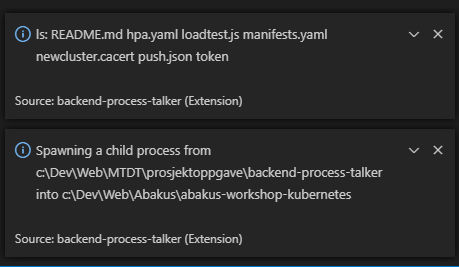
\includegraphics[width=.5\textwidth]{figures/vscode-extension-child_process-ls}
  \caption[VSCode Communicates with a Binary Executable]{VSCode executes a binary executable and displays its output.}\label{fig:prototype-1-ls}
\end{figure}

\paragraph*{Preparing a java jar file}
Next, a \texttt{.jar} file was creted from a java project.
This project was a separate one from the VSCode extension.
It would create an executable \texttt{.jar} which would echo back any text sent to its \emph{standard input}. The executable could also listen to a TCP port on \emph{localhost}, and echo back there.
For the \texttt{.jar} to be executable, the \texttt{main} method was registered in the \texttt{META-INF} file as the entry point.

\paragraph*{Running the jar in VSCode}
The code to execute \texttt{ls} was modified to run the \texttt{.jar} instead.
The \texttt{.jar} was placed in a (arbitrarily) named folder \emph{lib} in the VSCode extension project root.
To get the file path to the \texttt{.jar}, a \gls{VSCode} \acrshort{API} was used.
A code snipped illustrating this is shown in \cref{lst:prototype1-jar}.
Triggering the execution of the file was done using a \gls{VSCode} \emph{command} defined in the prototype, named \texttt{Hello World}.
Text was sent using standard input/output (\texttt{stdin, stdout}).
(Another version of the extension was also tried, sending data over TCP to a predefined port on \emph{localhost} (the same machine).)

\lstinputlisting[
    caption={Typescript code to run a java \texttt{.jar} in \gls{Nodejs}.},
    label=lst:prototype1-jar,
    language=Typescript
]{listings/run_jar_from_vscode.ts}

\paragraph*{Bundling the extension}
The last step is to create a bundle.
It is crucial that the bundle has the \texttt{.jar} file inside it, otherwise the extension would fail to run it, and this prototype would have a major problem.
A tool called \texttt{vsce} was installed and used.
This tool created a \texttt{.vsix} file, which is the extension installer.
Theia as VSCode needs this file, as it contains the prototype's code.
The \texttt{vsce} tool has a \texttt{ls} command, which shows all the files it will put into the bundle.
This command was executed, and the \texttt{.jar} file \emph{was} listed.

\paragraph*{Installing the extension}
Installation in VSCode is done by pressing \texttt{ctrl + shift + P} (on windows) and typing \texttt{>extensions: Install from vsix}, and then browsing to the file.
Installation in Theia is done by opening the \emph{Extensions} panel, and dragging the \texttt{.vsix} file into it.
The Theia instance used was in Gitpod with the \emph{Theia source code} workspace open\footnote{\href{https://gitpod.io/\#https://github.com/eclipse-theia/theia}{https://gitpod.io/\#https://github.com/eclipse-theia/theia}, requires login.}

\paragraph*{Activating the extension}
After installation, the Theia \emph{Commands} prompt was opened by pressing \texttt{F1} on the keyboard.
Then \texttt{Hello World} was entered, which is the name of the extension's \emph{command}.
Theia proceeded to show the outputs of the \texttt{.jar} file in a information popup.

\begin{figure}[htbp]  % order of priority: h here, t top, b bottom, p page
  \centering
  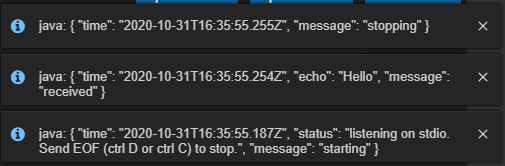
\includegraphics[width=.5\textwidth]{figures/theia-talks-to-jar-in-vscode-extension-via-stdio}
  \caption[Theia Executes a Bundled Jar File]{Theia is showing information popup windows that contain the outputs of executing a \texttt{.jar} file.}\label{fig:prototype1-theia-jar}
\end{figure}


\subsubsection{Results}
Because the extension resulted in a \texttt{.vsix} file with a \texttt{.jar} inside, and was installed and used in Theia successfully, the first prototype was a success.

The answer to \cref{rq:22} is:
\begin{displayquote}
  \emph{by bundling the java application as an executable \texttt{.jar}, and then starting it as a child process with the \gls{Nodejs} \acrshort{API} \texttt{child\_process.spawn}. Communication can be done from the Theia backend (or VSCode) over standard input/output or a network socket to a port on localhost.}
\end{displayquote}
  
This is based on the assumption that the \emph{host operating system has a java runtime installed and available on the path}.
However, this runtime \textit{could} be bundled itself.

Note that the Theia \emph{frontend} did \emph{not} communicate directly with the child process.
All communication was done by the backend and relayed to the frontend over \gls{JSON-RPC}.